\section{Introduction}
L'objectif du projet est d'implémenter un programme illustrant le concept de sécurité suivant : la stéganographie.\\

Abordée du point de vue du cours de système, elle nous permet d'approfondir nos connaissances sur l'utilisation de la mémoire
pour stocker des informations.\\

Il est évident que pour mener à bien un projet de cette envergure, d'autres compétences nous ont été nécessaires
telles que l'apprentissage approfondi du langage C, notamment pour réaliser des opérations de manipulation de bits.
Nous avons également eu besoin d'apprendre en détails les structures de fichier bitmap et GIF, pour décider de la meilleure technique à
utiliser afin d'y cacher des messages.\\

Dans ce rapport, nous passerons en revue l'organisation du projet, le choix pour chaque format et la technique utilisée. 
Nous fournirons aussi un guide pratique pour utiliser les exécutables. 

\vspace{1.5cm}

\newpage
\section{Organisation du projet}
La structure de notre projet s'organise essentiellement en quatre répertoires dont voici le détail :\\ 

\begin{itemize}
    \item \textbf{dist :} contient les exécutables du programme dans un dossier bmp et gif respectifs.
    \item \textbf{rapport :} contient le rapport en format tex et pdf, les fichiers qui serviront à construire celui-ci 
    ainsi que le makefile qui le lancera. On pourra également y trouver le document pdf de la présentation.
    \item \textbf{rsc :} contient les ressources qui servent d'input au programme [bitmap et gif] ainsi que les outputs 
    qui seront produits dans un dossier bmp et 
    gif respectifs.
    \item \textbf{src :} contient les sources du programme dans un dossier bmp et gif respectifs\\
\end{itemize}
On peut également trouver à la racine, un makefile général qui automatise le lancement du programme ainsi qu'un fichier README.

\vspace{1.5cm}
\section{Guide pratique}
\lstinputlisting[language=make, firstline=1, lastline=18]{../makefile}

\newpage
\section{Stéganographie : Définition}
La stéganographie est l'art de la dissimulation : son objet est de faire passer inaperçu des données dans d'autres données. 
Elle se distingue de la cryptographie, « art du secret », qui cherche à rendre un message inintelligible à autre que qui-de-droit.\\
Les fichiers peuvent être de type divers : fichiers image, audio, html, vidéos etc.\\
Parmi les scénarios de tests envisagés, nous avons tenté de cacher :\\

\begin{itemize}[label=$\diamond$, font=\LARGE \color{black}]
    \item un \textbf{texte} (.txt, .pdf) dans une \textbf{image} (.bmp/.gif)
    \item une \textbf{image} (.bmp, .gif) dans une \textbf{image} (.bmp/.gif)
    \item une \textbf{vidéo} (.mp4) dans une \textbf{image} (.bmp/.gif)\\
\end{itemize}

Il est évident que pour que cela soit possible, des conditions sont à poser.
Il faudra bien sûr que le fichier à cacher soit plus petit que le fichier objet. Il faudra aussi peauffiner les conditions de 
faisabilité qui sont fortement dépendantes du type de fichier et veiller à respecter la règle d'or : le dissimuler à tout prix.
Cela signifie qu'il faudra limiter au maximum l'impact sur le fichier dans lequel on aura caché des données sinon ce serait contraire
au principe de stéganographie.

\vspace{1.5cm}
\begin{center}
    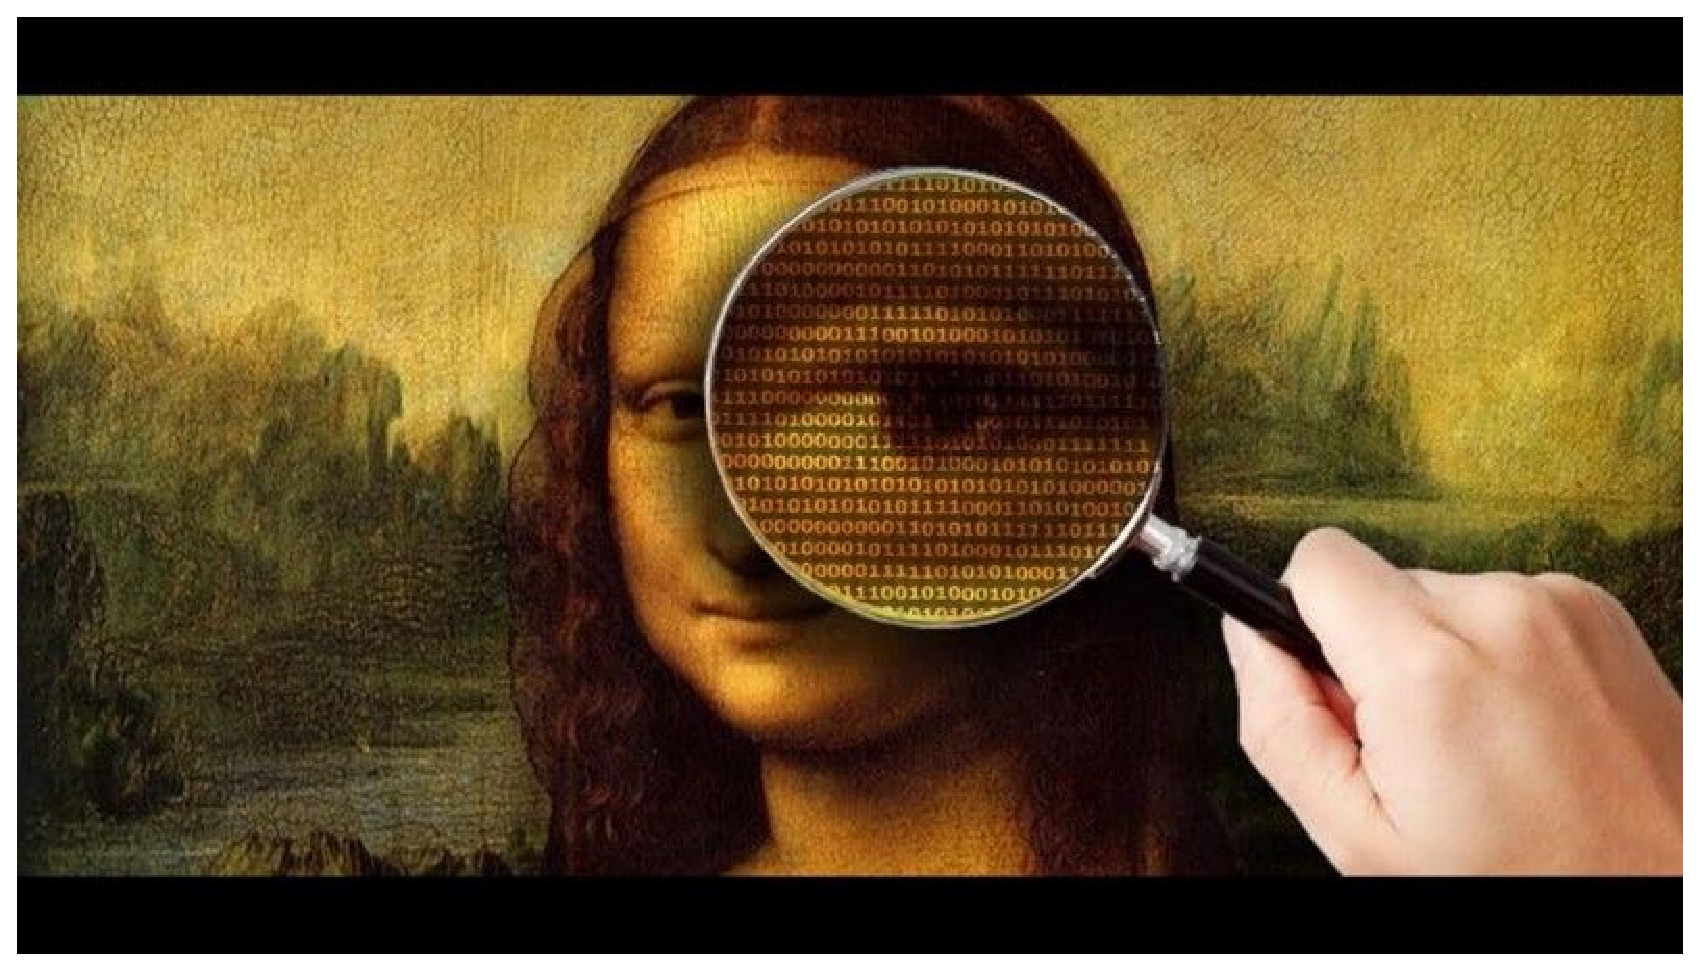
\includegraphics[width=10cm]{steganographie.eps}
\end{center}

\newpage
\section{Least Significant Bit (L.S.B.)}
Pour coder/décoder un message, nous employons la technique du Least Significant Bit (LSB). \\
Comme vous le voyez sur le schéma ci-dessous [Schéma général], cette technique consiste à se focaliser sur le bit le moins 
important d'un byte appelé le bit de poids faible.
Pour coder le message, il suffit de lire un byte à cacher et de l'encoder dans le bit de poids faible d'un byte choisi.
Pour décoder le message, il suffit de lire le bit de poids faible de ces bytes 'élus' et de reformer un message compréhensible.\\\\

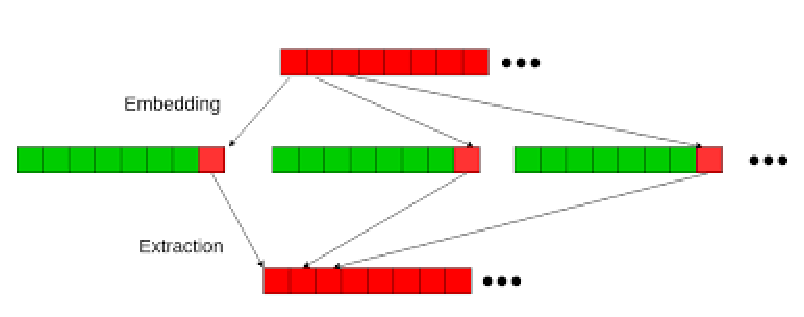
\includegraphics[width=15cm]{lsb.eps}\\

C'est cette logique que nous nous sommes employés à suivre dans le cas de traitement sur ces deux formats de fichiers image.
Ainsi, la technique est la même mais certains choix se sont imposés de part les différences entre les deux structures de ces 
fichiers image. Ces choix portent notamment sur 'l'élection' des bytes dans lesquels nous allons cacher l'information.
En effet, pour que le message ait le plus petit impact possible sur le fichier image, il faut employer des bytes qui peuvent
perdre un bit d'information sans que cela ne se remarque.
Par exemple, pour une couleur codée en rgb, le changement du dernier bit a un impact très faible, quasi invisible à l'oeil nu.
Il est donc adéquat pour y dissimuler des données.\\\\

\newpage
\subsection{Encodage : extrait de code source concernant la manipulation des LSB}
\lstinputlisting[language=c, firstline=57, lastline=72]{../src/utils/bmp.c}

\subsection{Décodage : extrait de code source concernant la manipulation des LSB}
\lstinputlisting[language=c, firstline=30, lastline=47]{../src/utils/bmp.c}
\lstinputlisting[language=c, firstline=92, lastline=95]{../src/utils/bmp.c}

